\documentclass[]{beamer}

\mode<presentation> {\usetheme{Warsaw}}

\usepackage{algorithm}
\usepackage[noend]{algorithmic}
%\usepackage[noend]{algpseudocode}
\usepackage{amstext}
\usepackage{amsmath,amsfonts,amssymb}
\usepackage{booktabs} % for professional tables
\usepackage{bm}

\usepackage[T1, T2A]{fontenc}    % use 8-bit T1 fonts
\usepackage[utf8]{inputenc} % allow utf-8 input
\usepackage[english]{babel}

\usepackage{animate}
\usepackage{citehack}
\usepackage{color}
\usepackage{enumerate}
\usepackage{epstopdf}
\usepackage{fontawesome}
\usepackage{geometry}
\usepackage{graphics, graphicx}
\usepackage{hyperref}       % hyperlinks
\usepackage{latexsym}
%\usepackage{lmodern}
\usepackage{mathtools}
\usepackage{mdframed}
\usepackage{microtype}      % microtypography
\usepackage{minted}
\usemintedstyle{default}
\usepackage{multirow}
\usepackage{nicefrac}       % compact symbols for 1/2, etc.
%\usepackage{pgfplots}
\usepackage{subfigure}
\usepackage{tikz}
\usetikzlibrary{patterns}
%\usepackage{times}
\usepackage{tgtermes}
\usepackage{url}            % simple URL typesetting
\usepackage{verbatim}

\epstopdfDeclareGraphicsRule{.gif}{png}{.png}{convert gif:#1 png:\OutputFile}
\AppendGraphicsExtensions{.gif}

%\addbibresource{references.bib}

\title[Analysis of approaches to uncertainty estimation]{\bfseries Investigation of the behavior of single-model uncertainty estimation approaches on large-scale tasks}
\author[Solotchii~M.]{Author: Mihail Solotchii \newline Advisors: Andrey Malinin, Artem Babenko}
\institute[CS HSE]{Master's thesis \\ Higher School of Economics, Faculty of Computer Science}
\date{June 8, 2021}

\setbeamertemplate{footline}[frame number]

\begin{document}

\begin{frame}
	\titlepage
\end{frame}

\begin{frame} \frametitle{Uncertainty estimation}
	\begin{itemize}
	    \item We want our model to make predictions along with some uncertainty measure \newline \par
	    \pause

	    \item We want uncertainty measures to correlate with quality of predictions \newline \par
	    \pause

		\item All theory behind ML models assumes the training and test distributions are the same \newline \par
		\pause

		\item We validate uncertainty estimation on Out-of-Distribution detection task (AUROC for quality measurement) \newline \par
	\end{itemize}
\end{frame}

\begin{frame} \frametitle{Known approaches}
    %ToDo: all methods in form of a tree \\
    %ToDo: literature \\
	\begin{itemize}
        \item Ensembles
        \begin{itemize}
            \item Measure models' disagreement
            \item Expensive \newline
        \end{itemize}
        \pause
	   % \item Distance-based models
	   % \begin{itemize}
	   %     \item Put objects in a latent space where objects reflect uncertainty
	   %     \item Not clear why they work \newline
	   % \end{itemize}
	   % \pause
	    \item Prior Networks
	    \begin{itemize}
            \item Emulate ensembles with a Dirichlet over predictions
            \item Need both ID and OoD data for training \newline
	    \end{itemize}
	    \pause
	    \item Evidential Networks
        \begin{itemize}
            \item Interpret networks' outputs as parameters of a Dirichlet
            \item Don't use OoD data on training
            \item Are tested using a simple architecture (LeNet) on simple datasets (e.g. MNIST)
	    \end{itemize}
	\end{itemize}
\end{frame}

\begin{frame} \frametitle{Goals and questions}
    \begin{itemize}
        \item Do Evidential models scale to large-scale tasks? \newline \par
        \item We need to understand this method better \\ (ideally, we would like to know why it works)
    \end{itemize}
\end{frame}

\begin{frame} \frametitle{Evidential Networks}
\begin{itemize}
    \item Parameters of a Dirichlet are inferred as follows
    $$\boldsymbol{\alpha} = \mathrm{ReLU}(f_{\boldsymbol{\theta}}(\boldsymbol{x})) + \boldsymbol{1}$$
    \item Uncertainty is measured by
    $$u(\boldsymbol{x}) = \frac{K}{\sum\limits_{j=1}^K \alpha_j(\boldsymbol{x})}$$
\end{itemize}
\end{frame}

% \begin{frame} \frametitle{Evidential Networks}
% \begin{itemize}
%     \item Last layer activation is ReLU (instead of softmax)
%     \item Loss function is cross-entropy + regularizer
%     $$\mathrm{P}(y = i | \boldsymbol{x}) = \frac{\alpha_i}{\sum\limits_{j=1}^K \alpha_j}$$
%     \item The loss function is
%     $$L(\boldsymbol{x}, \boldsymbol{y}) = \mathcal{L}(\boldsymbol{x}, \boldsymbol{y}) + \lambda \, \mathrm{KL} \Big( p(\boldsymbol{y} | \tilde{\boldsymbol{\alpha}}) \, || \, p(\boldsymbol{y} | \langle 1, \dots, 1 \rangle) \Big)$$
%     \item Uncertainty is measured by
%     $$u(\boldsymbol{x}) = \frac{1}{\sum\limits_{i=1}^K \alpha_i(\boldsymbol{x})}$$
% \end{itemize}
% \end{frame}

\begin{frame} \frametitle{Last-layer activation}
\begin{table}[H]
    \caption{Validation accuracy (\%)}
    \begin{center}
    \begin{small}
        \begin{tabular}{ l | c c c }
        \toprule
            Train dataset & Exponent & ReLU & Softplus \\
            \midrule
            CIFAR10  & \bf{96.17} & 59.31 & 95.79 \\
            CIFAR100 & \bf{81.00} & 32.17 & 67.30 \\
            \bottomrule
        \end{tabular}
    \end{small}
    \end{center}
\end{table}
\end{frame}

\begin{frame} \frametitle{Evidential Networks}
\begin{itemize}
    \item Parameters of a Dirichlet are now inferred as follows
    $$\boldsymbol{\alpha} = \mathrm{exp}(f_{\boldsymbol{\theta}}(\boldsymbol{x})) + \boldsymbol{1}$$
    \item Uncertainty is measured by
    $$u(\boldsymbol{x}) = \frac{K}{\sum\limits_{j=1}^K \exp\Big(f_{\boldsymbol{\theta}}(x) \Big) }$$
    \pause
    \item The loss function is
    $$L(\boldsymbol{x}, \boldsymbol{y}) = \mathcal{L}(\boldsymbol{x}, y) + \lambda \, R_{\mathrm{KL}}(\boldsymbol{x}, y)$$
\end{itemize}
\end{frame}

\begin{frame} \frametitle{Regularization and loss function}
\begin{table}[H]
    \begin{center}
    \caption{OOD detection performance (AUROC \%)}
    \begin{small}
    \begin{tabular}{ l l l | c c c | c c c }
        \toprule
        \multicolumn{2}{c}{Dataset} & \multirow{2}{*}{Reg} & \multicolumn{3}{c |}{EoE} & \multicolumn{3}{c}{MI} \\
        ID & OOD & & CE & Gibbs & $L_2$ & CE & Gibbs & $L_2$ \\
        \midrule
        \multirow{8}{*}{C100} & \multirow{2}{*}{SVHN} % CIFAR100 vs SVHN
        & On
        & 43.5 & 41.8 & 50.0
        & 39.0 & 47.6 & 50.0 \\
        & & Off
        & \bf{79.9} & 77.2 & 78.1
        & \bf{80.4} & 77.8 & 78.8 \\
        \cmidrule[0.5pt](lr){2-9}
        & \multirow{2}{*}{C10} % CIFAR100 vs CIFAR10
        & On
        & 51.6 & 59.2 & 50.0
        & 50.6 & 59.0 & 50.0 \\
        & & Off
        & \bf{81.3} & \bf{81.4} & 78.2
        & \bf{80.8} & \bf{81.1} & 77.0 \\
        \cmidrule[0.5pt](lr){2-9}
        & \multirow{2}{*}{LSUN} % CIFAR100 vs LSUN
        & On
        & 54.3 & 53.4 & 50.0
        & 56.6 & 57.2 & 50.0 \\
        & & Off
        & \bf{75.5} & \bf{75.8} & 71.3
        & \bf{74.0} & \bf{74.8} & 69.1 \\
        \cmidrule[0.5pt](lr){2-9}
        & \multirow{2}{*}{TiM} % CIFAR100 vs TinyImageNet
        & On
        & 51.2 & 58.4 & 50.0
        & 51.2 & 58.2 & 50.0 \\
        & & Off
        & \bf{81.7} & \bf{81.6} & 78.6
        & \bf{81.1} & \bf{81.1} & 76.6 \\
        \bottomrule
    \end{tabular}
    \end{small}
    \end{center}
\end{table}
\end{frame}

\begin{frame} \frametitle{Large-scale experiments}
\begin{table}[H]
    \begin{center}
    \caption{OOD detection performance (AUROC \%) on ImageNet}
    \begin{small}
        \begin{tabular}{ l l | c | c c }
            \toprule
            \multirow{2}{*}{ID set} & \multirow{2}{*}{OOD set} & \multicolumn{1}{c|}{Evidential} & \multicolumn{2}{c}{MI} \\
            & & Single & Single & Ens \\
            \midrule
            \multirow{8}{*}{ImNet-1k}
            & ImNet-O    & 58.1 % Evidential
                         & 57.4 & \bf{60.9} \\ % MI
            & ImNet-A    & 85.8 % Evidential
                         & 85.7 & \bf{87.0} \\ % MI
            & ImNet-R    & \bf{86.2} % Evidential
                         & 86.1 & 84.8 \\ % MI
            & ImNet-C1   & \bf{68.1} % Evidential
                         & 67.9 & 67.3 \\ % MI
            & ImNet-C2   & \bf{75.4} % Evidential
                         & \bf{75.3} & \bf{75.4} \\ % MI
            & ImNet-C3   & \bf{81.2} % Evidential
                         & \bf{81.1} & \bf{81.0} \\ % MI
            & ImNet-C4   & \bf{87.3} % Evidential
                         & \bf{87.3} & 86.0 \\ % MI
            & ImNet-C5   & \bf{91.6} % Evidential
                         & \bf{91.6} & 88.4 \\ % MI
            \bottomrule
        \end{tabular}
    \end{small}
    \end{center}
\end{table}
\end{frame}

% \begin{frame} \frametitle{Evidential method is a kernel method}
% \begin{center}
%     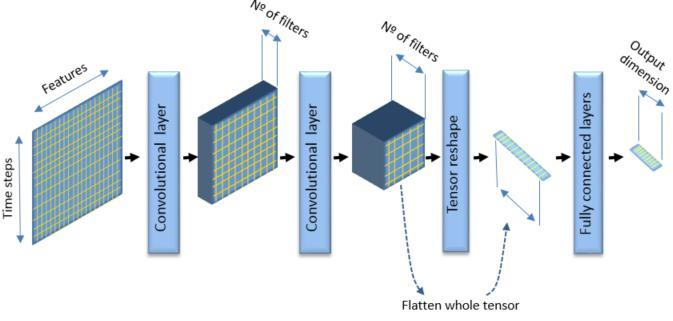
\includegraphics[scale=0.5]{Deep-learning-CNN-model.jpg}
% \end{center}
% $$\frac{1}{u(\boldsymbol{W}, \boldsymbol{e})} = K(\boldsymbol{W}, \boldsymbol{e}) = \sum\limits_{i=1}^K \exp(\langle \boldsymbol{w}_i, \boldsymbol{e} \rangle)$$
% \end{frame}

\begin{frame} \frametitle{Embedding space}
\begin{figure}[H]
    \caption{Representations of the network's penultimate layer reduced to 2 dimensions with t-SNE}
    \centering
    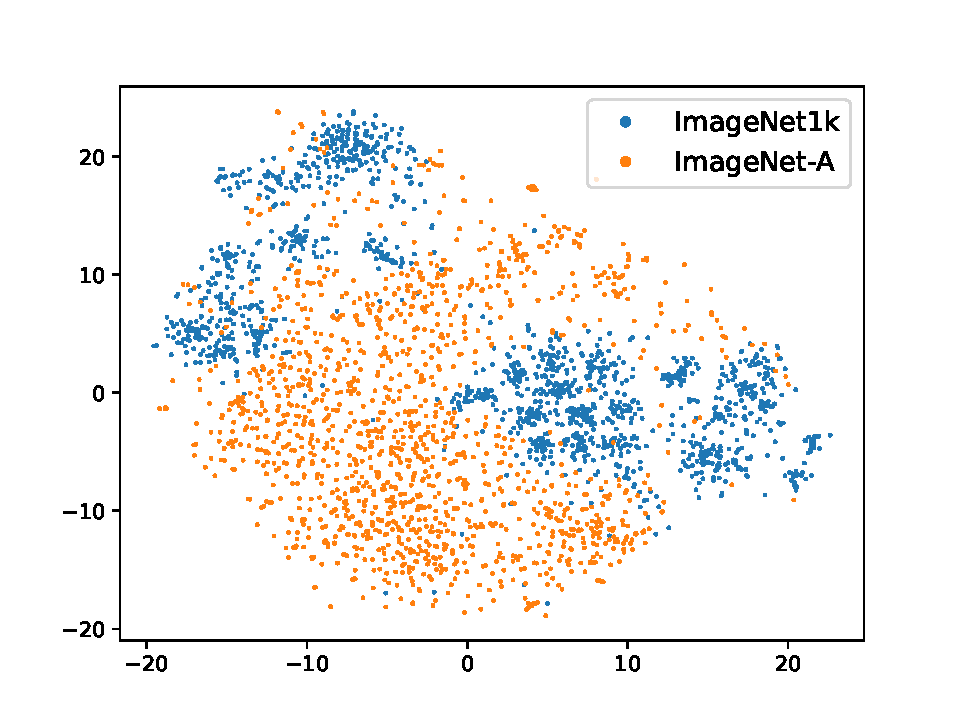
\includegraphics[scale=0.5]{tsne_1k_A.pdf}
\end{figure}
\end{frame}

\begin{frame} \frametitle{Maximum cosine correlation with model performance}
\begin{table}[H]
    \caption{Confidence measures and model performance on ImageNet-C}
    \begin{center}
    \begin{small}
        \begin{tabular}{ l | c c c c c c }
            \toprule
            Corruption level & C0 & C1 & C2 & C3 & C4 & C5 \\
            \midrule
            Evidential
            & 17.4 & 14.4 & 13.1 & 12.0 & 10.8 & 10.0 \\
            Maximum cosine
            & 0.45 & 0.38 & 0.35 & 0.32 & 0.29 & 0.27 \\
            Model accuracy (\%)
            & 75.9 & 59.7 & 48.7 & 38.4 & 27.1 & 17.8 \\
            \bottomrule
        \end{tabular}
    \end{small}
    \end{center}
\end{table}
\end{frame}

% \begin{frame} \frametitle{Maximum cosine}
% \begin{figure}[H]
%     \caption{Distribution of sorted cosines for ID and OoD data points}
%     \centering
%     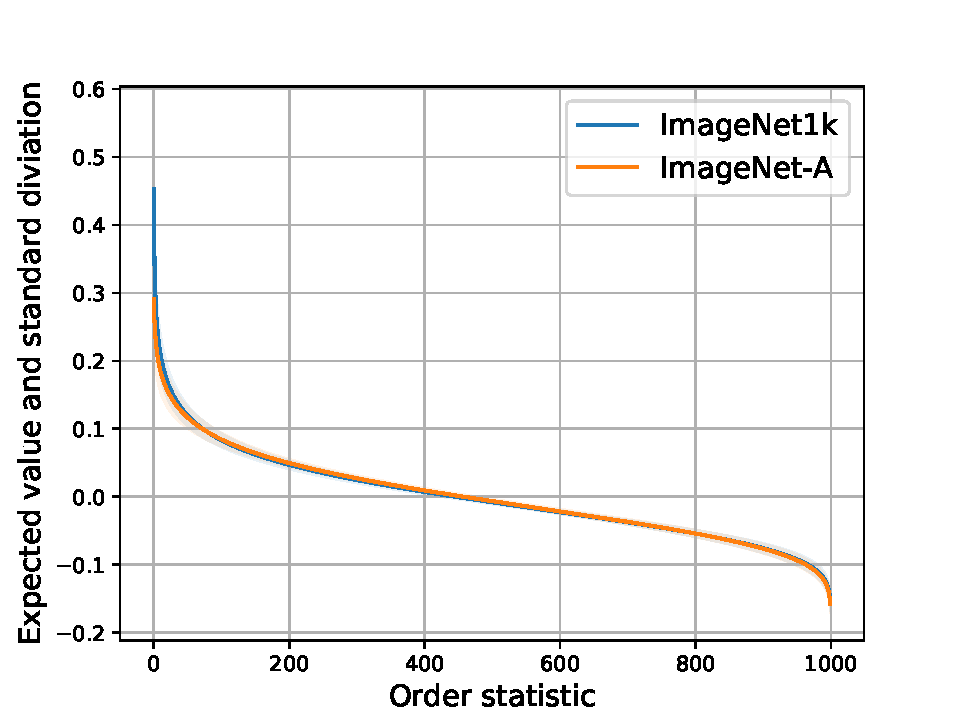
\includegraphics[scale=0.5]{cosines_sorted_mean_ImageNet1k-A.pdf}
% \end{figure}
% \end{frame}

\begin{frame} \frametitle{Maximum cosine}
\begin{figure}[H]
    \caption{{\color{blue} ID embeddings} and {\color{orange} OoD embeddings} around the prototypes (arrows)}
    \vspace{-8pt}
    \centering
    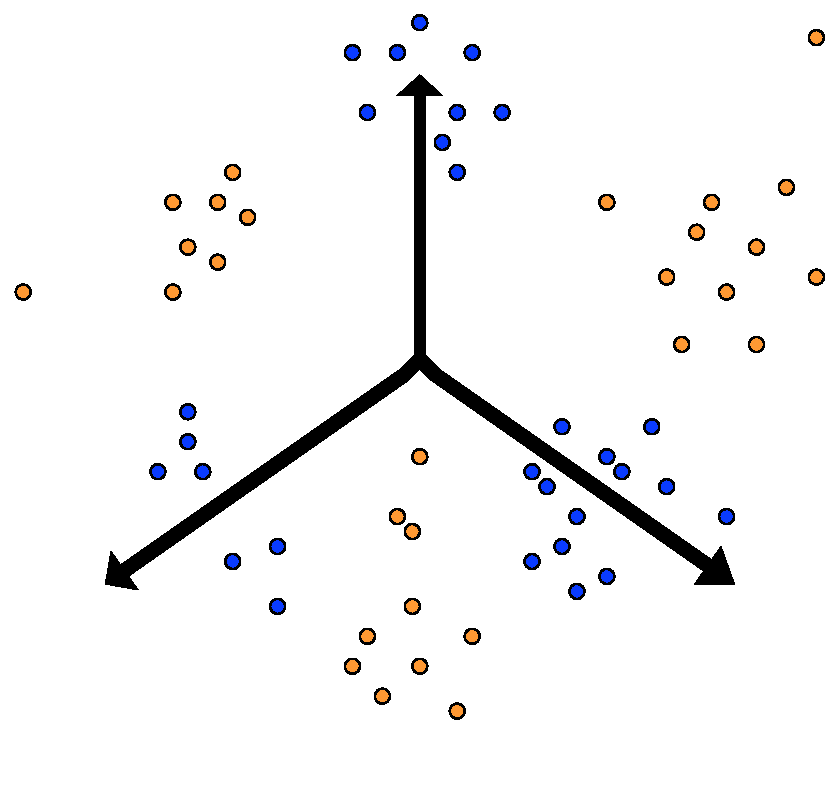
\includegraphics[scale=0.45]{circle.pdf}
\end{figure}
\end{frame}

\begin{frame} \frametitle{Large-scale experiments}
\begin{table}[H]
    \begin{center}
    \caption{OOD detection performance (AUROC \%) on ImageNet}
    \begin{small}
        \begin{tabular}{ l l | c | c | c c }
            \toprule
            \multirow{2}{*}{ID set} & \multirow{2}{*}{OOD set} & \multicolumn{1}{c|}{MaxCos} & \multicolumn{1}{c|}{Evidential} & \multicolumn{2}{c}{MI} \\
            & & Single & Single & Single & Ens \\
            \midrule
            \multirow{8}{*}{ImNet-1k}
            & ImNet-O    & \bf{68.0} % Max cosine
                         & 58.1 % Evidential
                         & 57.4 & 60.9 \\ % MI
            & ImNet-A    & \bf{88.1} % Max cosine
                         & 85.8 % Evidential
                         & 85.7 & 87.0 \\ % MI
            & ImNet-R    & \bf{87.1} % Max cosine
                         & \bf{86.2} % Evidential
                         & 86.1 & 84.8 \\ % MI
            & ImNet-C1   & 66.7 % Max cosine
                         & \bf{68.1} % Evidential
                         & 67.9 & 67.3 \\ % MI
            & ImNet-C2   & 74.6 % Max cosine
                         & \bf{75.4} % Evidential
                         & \bf{75.3} & \bf{75.4} \\ % MI
            & ImNet-C3   & 80.5 % Max cosine
                         & \bf{81.2} % Evidential
                         & \bf{81.1} & \bf{81.0} \\ % MI
            & ImNet-C4   & 86.4 % Max cosine
                         & \bf{87.3} % Evidential
                         & \bf{87.3} & 86.0 \\ % MI
            & ImNet-C5   & 90.6 % Max cosine
                         & \bf{91.6} % Evidential
                         & \bf{91.6} & 88.4 \\ % MI
            \bottomrule
        \end{tabular}
    \end{small}
    \end{center}
\end{table}
\end{frame}

\begin{frame}{Conclusions}
\begin{itemize}
    \item Do Evidential methods scale?
    \begin{itemize}
        \item Evidential methods as they are do not scale
        \item A simple modification to Evidential methods does scale \newline
    \end{itemize}
    \pause
    \item Properties of the method:
    \begin{itemize}
        \item ID embeddings are closer to the prototypes by cosine distance
        \item Maximum cosine between an embedding and prototypes is a good OoD detector
    \end{itemize}
\end{itemize}    
\end{frame}

\end{document}